\documentclass[11pt,professionalfonts,hyperref={pdftex,pdfpagemode=none,pdfstartview=FitH}]{beamer}
%\usepackage{times}
%\usefonttheme{serif}
%\usepackage{helvet}
%\usepackage{amsmath,amssymb}
\usepackage{graphicx,multirow}

\usepackage{movie15}

\usepackage{caption}
\usepackage{subcaption}
\captionsetup{compatibility=false}

%\usepackage{warmread}
%\usepackage[all,import]{xy}

%\renewcommand\mathfamilydefault{\rmdefault}

% JIRS includes
%\usepackage{graphicx}
%\usepackage{amsmath,amssymb,url,times}%,subfigure}% amsthm is the one!
%\usepackage{caption,subcaption,hyperref}
%\usepackage{color,comment}
%\usepackage{curves,pgfgantt}

\newcommand{\norm}[1]{\ensuremath{\left\| #1 \right\|}}
\newcommand{\bracket}[1]{\ensuremath{\left[ #1 \right]}}
\newcommand{\braces}[1]{\ensuremath{\left\{ #1 \right\}}}
\newcommand{\parenth}[1]{\ensuremath{\left( #1 \right)}}
\newcommand{\pair}[1]{\ensuremath{\langle #1 \rangle}}
\newcommand{\met}[1]{\ensuremath{\langle\langle #1 \rangle\rangle}}
\newcommand{\refeqn}[1]{(\ref{eqn:#1})}
\newcommand{\reffig}[1]{Fig. \ref{fig:#1}}
\newcommand{\tr}[1]{\mathrm{tr}\ensuremath{\negthickspace\bracket{#1}}}
\newcommand{\trs}[1]{\mathrm{tr}\ensuremath{[#1]}}
\newcommand{\deriv}[2]{\ensuremath{\frac{\partial #1}{\partial #2}}}
\newcommand{\SO}{\ensuremath{\mathsf{SO(3)}}}
\newcommand{\T}{\ensuremath{\mathsf{T}}}
\renewcommand{\L}{\ensuremath{\mathsf{L}}}
\newcommand{\so}{\ensuremath{\mathfrak{so}(3)}}
\newcommand{\SE}{\ensuremath{\mathsf{SE(3)}}}
\newcommand{\se}{\ensuremath{\mathfrak{se}(3)}}
\renewcommand{\Re}{\ensuremath{\mathbb{R}}}
\newcommand{\aSE}[2]{\ensuremath{\begin{bmatrix}#1&#2\\0&1\end{bmatrix}}}
\newcommand{\ase}[2]{\ensuremath{\begin{bmatrix}#1&#2\\0&0\end{bmatrix}}}
\newcommand{\D}{\ensuremath{\mathbf{D}}}
\newcommand{\Sph}{\ensuremath{\mathsf{S}}}
\renewcommand{\S}{\Sph}
\newcommand{\J}{\ensuremath{\mathbf{J}}}
\newcommand{\Ad}{\ensuremath{\mathrm{Ad}}}
\newcommand{\intp}{\ensuremath{\mathbf{i}}}
\newcommand{\extd}{\ensuremath{\mathbf{d}}}
\newcommand{\hor}{\ensuremath{\mathrm{hor}}}
\newcommand{\ver}{\ensuremath{\mathrm{ver}}}
\newcommand{\dyn}{\ensuremath{\mathrm{dyn}}}
\newcommand{\geo}{\ensuremath{\mathrm{geo}}}
\newcommand{\Q}{\ensuremath{\mathsf{Q}}}
\newcommand{\G}{\ensuremath{\mathsf{G}}}
\newcommand{\g}{\ensuremath{\mathfrak{g}}}
\newcommand{\Hess}{\ensuremath{\mathrm{Hess}}}
\newcommand{\refprop}[1]{Proposition \ref{prop:#1}}
\newcommand{\argmax}{\operatornamewithlimits{argmax}}

\definecolor{mygray}{gray}{0.9}

\mode<presentation> {
  \usetheme{Warsaw}
  \usefonttheme{serif}
  \setbeamercovered{transparent}
}

\newcommand{\mypaper}{}

\setbeamertemplate{footline}%{split theme}
{%
  \leavevmode%
  \hbox{\begin{beamercolorbox}[wd=.9\paperwidth,ht=2.5ex,dp=1.125ex,leftskip=.3cm,rightskip=.3cm plus1fill]{author in head/foot}%
    \usebeamerfont{author in head/foot}\insertshorttitle
  \end{beamercolorbox}%
  \begin{beamercolorbox}[wd=.1\paperwidth,ht=2.5ex,dp=1.125ex,leftskip=.3cm,rightskip=.3cm plus1fill]{title in head/foot}
    \usebeamerfont{title in head/foot}\mypaper\hfill \insertframenumber/\inserttotalframenumber
  \end{beamercolorbox}}%
  \vskip0pt%
} \setbeamercolor{box}{fg=black,bg=yellow}

\title[Autonomous Exploration by Expected Information Gain from Prob. Occupancy Grid Mapping]
{\large Autonomous Exploration by Expected Information Gain from Probabilistic Occupancy Grid Mapping}

\author{\vspace*{-0.3cm}}

\institute{\footnotesize
{\normalsize Evan Kaufman, Taeyoung Lee, and Zhuming Ai}\vspace*{0.2cm}\\
  Mechanical and Aerospace Engineering\\ George Washington University \vspace*{0.6cm}\\ {\normalsize Special Thanks to Ira. S. Moskowitz and Mark Livingston} \vspace*{0.2cm}\\Information Management \& Decision Architectures\\U.S. Naval Research Laboratory}

\date{}

\definecolor{tmp}{rgb}{0.804,0.941,1.0}
\setbeamercolor{numerical}{fg=black,bg=tmp}
\setbeamercolor{exact}{fg=black,bg=red}

\newtheorem{prop}{Proposition}



\renewcommand{\emph}[1]{\textit{\textbf{\color{blue}{#1}}}}


\begin{document}

\begin{frame}
  \titlepage
\end{frame}


\section*{}
\subsection*{Background and Motivation}

\begin{frame}
\frametitle{Motivation}
\begin{itemize}
	\item Building Maps and Exploration
	\begin{itemize}
		\item Search and rescue: quickly building a map and finding targets in places with physical or health hazards
		\item Surveillance: gather information of enemy locations
    		\item Convenience: autonomous robotic cleaning
	\end{itemize}
	\pause
	\item Goals
	\begin{itemize}
		\item Build \emph{accurate} probabilistic maps
		\item Use map properties to \emph{predict} how the \emph{map information} will change with various actions
		\item Motion planning for \emph{collision-free} trajectories
		\item Generate algorithms capable of \emph{real-time} implementation
	\end{itemize}
\end{itemize}

\only<1->{
\begin{figure}
\centerline{
    \includegraphics[height=2.1cm]{ogm_ex3.jpeg}\hspace*{0.1cm}
\hspace*{0.5cm}
    \includegraphics[height=2.1cm]{ogm_ex1.jpg}\hspace*{0.1cm}
\hspace*{0.5cm}
    \includegraphics[height=2.1cm]{ogm_ex2.png}\hspace*{0.1cm}
}
\end{figure}}
\end{frame}


\begin{frame}
\frametitle{Background: Occupancy Grid Mapping}
	\begin{itemize}
		\item Environment decomposed into evenly-space grid cells
		\item \emph{Binary} random variable: cells are either \emph{occupied} or \emph{free}
		\item Sensor reading $z$, the \emph{forward sensor model} is $p(z|m,X)$ is the measurement probability density, assuming the stochastic properties are known
		\begin{figure}[!htbp]
		\vspace*{-0.0cm}
		%\vspace*{0.25cm}
		\centerline{
	  	  \includegraphics[width=7cm]{BeamModel.png}\hspace*{0.1cm}
	    	}
		\vspace*{0.25cm}
		\centerline{
	    	\includegraphics[width=5cm]{1D_True_Grid.png}\hspace*{0.1cm}
		%    \hspace*{0.75cm}
	    	}
		{Beam Model for Range Finders}
	\end{figure}
	    	\item Goal: generate a \emph{probabilistic} map $m$ given robot pose $X$
	\end{itemize}
\end{frame}


\begin{frame}
\frametitle{Background: Occupancy Grid Mapping}
	\begin{itemize}
		\item Cell occupancy probabilities obtained using the \emph{inverse sensor model}, $P(m|z,X)$, which gives grid cell probabilities based on the latest measurement $z$
		\item The exact inverse sensor model was believed to require $\mathcal O(2^n)$ for \emph{each} grid cell within the sensor field of view, so popular substitutes were \emph{heuristic} or \emph{learned} solutions
		\item Recently, the exact inverse sensor model was solved in real-time by grouping map outcomes
		\begin{figure}[!htbp]
		\vspace*{0.5cm}
		\centerline{
			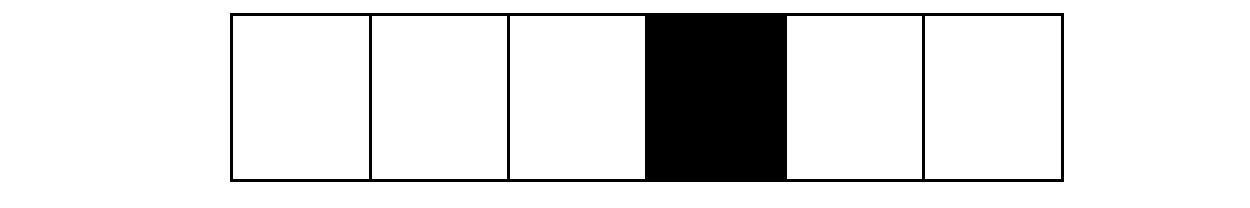
\includegraphics[width=4.0cm]{rkplus_1.png}\hspace*{-0.5cm}
			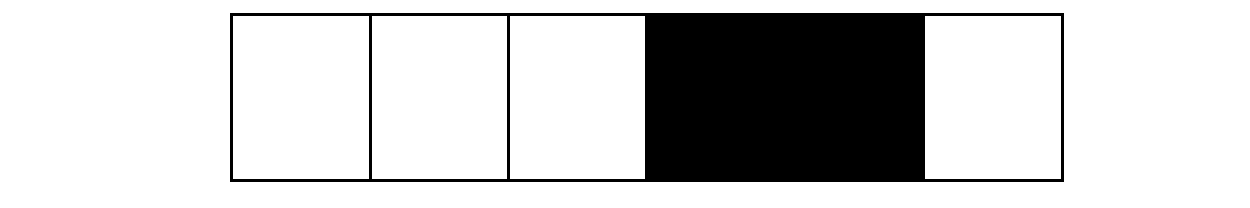
\includegraphics[width=4.0cm]{rkplus_2.png}}
		 \centerline{
		\includegraphics[width=4.0cm]{rkplus_3.png}\hspace*{-0.5cm}
		\includegraphics[width=4.0cm]{rkplus_4.png}}
		\end{figure}
		\item By grouping, the inverse sensor model requires $\mathcal O(n+1)$, compared with $\mathcal O(2^n)$: applied in \emph{real-time}
	\end{itemize}
\end{frame}


% check here
%\begin{frame}
%\frametitle{Exact Occupancy Grid Mapping: Hallway Comparison}
%	\begin{itemize}
%		\item Comparison between approximate and exact results
%		\begin{figure}[!htbp]
%		    \centering
%		    \begin{subfigure}{.45\textwidth}
%		        \centering
%		        \includegraphics[width=\textwidth]{map_comparison.png}
%		        \caption*{Occupancy Grid Map}
%		    \end{subfigure}
%		    \hspace*{-.05\textwidth}
%		    \begin{subfigure}{.45\textwidth}
%		        \centering
%		        \includegraphics[width=\textwidth]{map_zoom.png}
%		        \caption*{Zoomed In Map}
%		    \end{subfigure}
%		\end{figure}
%	\end{itemize}
%\end{frame}


\begin{frame}
\frametitle{Exact Occupancy Grid Mapping: Hallway Comparison}
\begin{minipage}[t]{0.4\textwidth}
\begin{itemize}
	\item Occupancy grid mapping using an approximate and the exact solution are compared
	\item Both algorithms subject to the same pose and measurement sets 
	\item The exact algorithm yields a more \emph{certain} map shown with entropy $H$ (blue: certain, red: uncertain)
\end{itemize}
\end{minipage}
	\begin{minipage}[t]{0.5\textwidth}
		\begin{figure}[!htbp]
		    \centering
		    \begin{subfigure}{0.5\textwidth}
		        \centering
		        \includegraphics[width=.8\textwidth]{AISM_Image_19.pdf}
		        \caption*{Approx. $P(m)$}
		    \end{subfigure}
		    \hspace*{-0.1\textwidth}
		    \begin{subfigure}{0.5\textwidth}
		        \centering
		        \includegraphics[width=.8\textwidth]{EISM_Image_19.pdf}
		        \caption*{Exact $P(m)$}
		    \end{subfigure}
		\end{figure}
		\vspace*{-.1\textwidth}
		\begin{figure}[!htbp]
		    \centering
		    \begin{subfigure}{0.5\textwidth}
		        \centering
		        \includegraphics[width=.8\textwidth]{AISM_Image_inf_19.pdf}
		        \caption*{Approx. $H$}
		    \end{subfigure}
		    \hspace*{-0.1\textwidth}
		    \begin{subfigure}{0.5\textwidth}
		        \centering
		        \includegraphics[width=.8\textwidth]{EISM_Image_inf_19.pdf}
		        \caption*{Exact $H$}
		    \end{subfigure}
		\end{figure}
	\end{minipage}


%	\begin{itemize}
%		\item The exact algorithm yields a more \emph{certain} map from the same measurement set
%		\begin{figure}[!htbp]
%		    \centering
%		    \begin{subfigure}{0.5\textwidth}
%		        \centering
%		        \includegraphics[width=.5\textwidth]{AISM_Image_inf_19.pdf}
%		        \caption*{Approximate}
%		    \end{subfigure}
%		    \hspace*{-0.1\textwidth}
%		    \begin{subfigure}{0.5\textwidth}
%		        \centering
%		        \includegraphics[width=0.5\textwidth]{EISM_Image_inf_19.pdf}
%		        \caption*{Exact}
%		    \end{subfigure}
%		\end{figure}
%	\end{itemize}
\end{frame}


\section*{}
\subsection*{Autonomous Exploration}


\begin{frame}
\frametitle{Autonomous Exploration Description}
\begin{itemize}
        \item The environment is initially unknown, so the robot path is initially uncertain
	\item Simultaneous localization and mapping assumes robotic actions are provided
	\item Human interaction is common to guide the robot
	\item Goal: develop effective policies to govern robotic motion that generates a map accurately and efficiently
\end{itemize}

\end{frame}



\begin{frame}
\frametitle{Background: Autonomous Exploration}
\begin{itemize}
        	\item Uncertainty-Based Exploration
	\begin{itemize}
		\item Main idea: choose robot motions that minimize the uncertainty of the occupancy grid map
		\item Equivalently maximize map information gain
	\end{itemize}
\end{itemize}
\begin{minipage}[t]{7.0cm}
\begin{itemize}
	\item Entropy
	\begin{itemize}		
		\item \emph{Shannon's entropy} serves as an uncertainty measure
		\begin{align*}
			H(P)=-P\log P-\bar{P}\log \bar{P}%-(1-P)\log(1-P)
		\end{align*}
		with cell occupancy probability $P$ and complement $\bar{P}=1-P$
		\item Entropy $H$ is maximized when $P=0.5$ and minimized as $P\rightarrow0$ or $P\rightarrow1$
	\end{itemize}
\end{itemize}
\end{minipage}
\begin{minipage}[t]{3.0cm}
\vspace*{0.5cm}
\begin{figure}[!htbp]
	\centerline{
		\hspace*{1.25cm}
   		\includegraphics[width=5.0cm]{H_Plotted_square.pdf}%\hspace*{0.1cm}
	}
\end{figure}
\end{minipage}

\end{frame}


\begin{frame}
\frametitle{Problem Definition}
\begin{itemize}
        	\item Map Information Gain Maximization
	\begin{itemize}
		\item Goal: choose a set of optimal future poses to maximize map information gain
		\pause
		\item Challenge: the complete set cannot be calculated accurately with an initially highly-uncertain environment
		\pause
		\item Solution: choose short-term optimal pose goals, reevaluating an updated map for the subsequent optimizations
		\pause
		\item The information gain considering candidate future pose $X_c$:% is
		\begin{align*}
			\mathcal I(X_c)&=H(P(m|X_{1:t},Z_{1:t}))-\text{E}\left[H(P(m|X_{1:t},Z_{1:t},X_c,Z_c))\right]
		\end{align*}
		\pause
		\item Optimal pose $X^*_c$ satisfies
		\begin{align*}
			X_c^*=\argmax_{X_c}{\mathcal I(X_c)}
		\end{align*}
	\end{itemize}
\end{itemize}


\end{frame}



\begin{frame}
\frametitle{Related Work}
\begin{itemize}
        	\item Frontier-Based Exploration
	\begin{itemize}
		\item Main idea: robot moves toward boundaries between certain and uncertain space, takes measurements, then pushes back the boundaries
		\item Typically not based directly on grid cell entropy
		\item Heuristic
	\end{itemize}
	\pause
	\item Entropy-Based Exploration
	\begin{itemize}
		\item Cell occupancy probabilities are inaccurate: inverse sensor model is heuristic or learned, and frequently estimated with Rao-Blackwellized particle filters
		\item Inaccurate probabilities imply inaccurate entropy measures
		\item Approaches use ``hallucination measurements'' to predict how future measurements \emph{might} affect the map uncertainty,
		\begin{align*}
			\text{E}\left[H(P(m|X_{1:t},Z_{1:t},X_c,Z_c))\right]\approx H(P(m|X_{1:t},Z_{1:t},X_c,\text{E}\left[Z_c\right]))
		\end{align*}
	\end{itemize}
\end{itemize}


\end{frame}


\begin{frame}
\frametitle{Direct Entropy Calculation}
\begin{itemize}
        \item Instead of relying on frontiers or making assumptions about measurements, the expected map entropy is \emph{calculated directly} by the expected value:
	\begin{align*}
		\text{E}[H(P(m|X,z))]=\int_{z_\text{min}}^{z_\text{max}}
		H(P(m|X,z))p(z|X)dz,
	\end{align*}
	\pause
	\item The integral is discretized by intersections between the measurement and grid cells:
	\begin{align*}
		\text{E}[H(P(m|X,z))]=\sum_{k=1}^{n+1}\bigg\{H(P(m|X,z_k))P(z_{k}|X)\bigg\}
	\end{align*}
	\pause
	\item Entropy $H(P(m|X,z_k))$ is obtained with the exact inverse sensor model and definition of entropy
	\item Probability $P(z_{k}|X)$ is obtained with normalizing values from the exact inverse sensor model
\end{itemize}


\end{frame}


\begin{frame}
\frametitle{Direct Entropy Calculation: Computational Challenges}
\begin{itemize}
        \item Problem: $\text{E}[H(P(m|X,z))]$ requires $\mathcal O((n+1)^2)$ for $n+1$ possible measurement outcomes: measurement detects any of the $n$ cells or returns a maximum reading
        \pause
        \item Solution: select the $\hat n$ most probable outcomes for $\mathcal O(\hat n^2)$
        \pause
        \item Monte Carlo simulations ($100$ trials) to determine the expected entropy of a measurement ray compare the exact and approximate resulting accuracies and times
\end{itemize}

		\begin{figure}[!htbp]
		    \centering
		    \begin{subfigure}{0.5\textwidth}
		        \centering
		        \includegraphics[width=.8\textwidth]{simpar_approx_err.pdf}
		        \caption*{Error}
		    \end{subfigure}
		    \hspace*{-0.1\textwidth}
		    \begin{subfigure}{0.5\textwidth}
		        \centering
		        \includegraphics[width=.8\textwidth]{simpar_approx_t.pdf}
		        \caption*{Time Ratio}
		    \end{subfigure}
		\end{figure}

\end{frame}



\begin{frame}
\frametitle{Pose Selection}

\begin{minipage}[t]{7.0cm}
\begin{itemize}
	\item Several locations serve as candidates for the robot to move toward
	\item The optimal attitude at each location maximized expected information gain
	\item The pose (location and attitude) with the largest overall expected information gain is selected
	\item Other costs, such as distance or travel time, can be included in the optimization
\end{itemize}
\end{minipage}
\begin{minipage}[t]{3.0cm}
\vspace*{0.5cm}
\begin{figure}[!htbp]
	\centerline{
		\hspace*{1.0cm}
   		\includegraphics[width=5.0cm]{pose_selection}%\hspace*{0.1cm}
	}
\end{figure}
\end{minipage}


\end{frame}


\begin{frame}
\frametitle{Collision-Free Path}

\begin{itemize}
	\item \emph{Waypoints}
	\begin{itemize}
		\item Using the grid map as the graph, \emph{Dijkstra's algorithm} provides collision-free waypoints for the robot path
		\item Probability of collision at pose $X$ must be within threshold $\beta>0$,
		\begin{align*}
			P_\text{collision}(X)=1-\prod_{i\in\mathcal C_X}P(\bar{\mathbf{m}}_i|X_{1:t},Z_{1:t})\leq\beta
		\end{align*}
	\end{itemize}
	\pause
	\item \emph{Constrained Polynomial Least Squares}
	\begin{itemize}
		\item Smooth trajectory as a function of time minimizes the squared error between the curve and the waypoints
		\item Constrained to beginning and terminal poses
		\item For complicated trajectories, splines are patched together by constraining position and velocity at the connection
	\end{itemize}
\end{itemize}


\end{frame}



	


\begin{frame}
\frametitle{Numerical Example}
\begin{itemize}
        	\item A benchmark example floor plan is explored and mapped using the proposed mapping and exploration algorithms
	\item Simulations in Robot Operating System (ROS)
\end{itemize}
\begin{figure}
    \centering
    \includegraphics[width=0.4\textwidth]{intel_clean.png}
    \caption*{Modified Intel Research Lab floor plan form the SLAM benchmark}
\end{figure}

\end{frame}

%% VIDEO 1: Simulation %%
\begin{frame}
%\href{run:JIRS16_simulation_speedup10x_then_speedup100x.mov}{Simulation Video Link}
\frametitle{Numerical Results}
	\centering{
	\includemovie[poster,autoplay]{\textwidth}{0.66667\textwidth}{JIRS16_simulation_speedup10x_then_speedup100x.mov}}
\end{frame}

\begin{frame}
\frametitle{Numerical Results}

\begin{figure}[!ht]
    \centering
    \begin{subfigure}[t]{0.2\columnwidth}
        \centering
        \includegraphics[trim = {4.6cm 3.8cm 4.6cm 0}, clip, width=\textwidth]{0min.png}
        \caption*{$t=0$ min}
        \label{fig:IRL0min}
    \end{subfigure}
    \begin{subfigure}[t]{0.2\columnwidth}
        \centering
        \includegraphics[trim = {4.6cm 3.8cm 4.6cm 0}, clip, width=\textwidth]{5min.png}
        \caption*{$t=5$ min}
        \label{fig:IRL5min}
    \end{subfigure}
    \begin{subfigure}[t]{0.2\columnwidth}
           \centering
           \includegraphics[trim = {4.6cm 3.8cm 4.6cm 0}, clip, width=\textwidth]{10min.png}
        \caption*{$t=10$ min}
        \label{fig:IRL10min}
    \end{subfigure}
    \begin{subfigure}[t]{0.2\columnwidth}
           \centering
           \includegraphics[trim = {4.6cm 3.8cm 4.6cm 0}, clip, width=\textwidth]{15min.png}
        \caption*{$t=15$ min}
        \label{fig:IRL15min}
    \end{subfigure}
    \begin{subfigure}[t]{0.2\columnwidth}
         \centering
         \includegraphics[trim = {4.6cm 3.8cm 4.6cm 0}, clip, width=\textwidth]{20min.png}
        \caption*{$t=20$ min}
        \label{fig:IRL20min}
    \end{subfigure}
    \begin{subfigure}[t]{0.2\columnwidth}
           \centering
           \includegraphics[trim = {4.6cm 3.8cm 4.6cm 0}, clip, width=\textwidth]{25min.png}
        \caption*{$t=25$ min}
        \label{fig:IRL25min}
    \end{subfigure}
    \begin{subfigure}[t]{0.2\columnwidth}
           \centering
           \includegraphics[trim = {4.6cm 3.8cm 4.6cm 0}, clip, width=\textwidth]{30min.png}
        \caption*{$t=30$ min}
        \label{fig:IRL30min}
    \end{subfigure}
    \begin{subfigure}[t]{0.2\columnwidth}
           \centering
           \includegraphics[trim = {4.6cm 3.8cm 4.6cm 0}, clip, width=\textwidth]{35min.png}
        \caption*{$t=35$ min}
        \label{fig:IRL35min}
    \end{subfigure}
%    \begin{subfigure}[t]{0.2\columnwidth}
%           \centering
%           \includegraphics[trim = {4.6cm 3.8cm 4.6cm 0}, clip, width=\textwidth]{40min.png}
%        \caption*{$t=40$ min}
%        \label{fig:IRL40min}
%    \end{subfigure}
\vspace*{-0.25cm}
    \caption*{A robot (green) measures a room in ROS Stage simulator using modified Intel Research Lab floor plan using the proposed mapping and exploration algorithms. \href{run:JIRS16_simulation_speedup10x_then_speedup100x.mov}{(Simulation Video Link)}
}
    \label{fig:IRL}
\end{figure}
\href{run:JIRS16_simulation_speedup10x_then_speedup100x.mov}{Simulation Video Link}



\end{frame}





\begin{frame}
\frametitle{Experimental Example}
\begin{itemize}
        	\item A pioneer ground vehicle explores a room composed of Styrofoam walls
	\item Experiments use ROS, a Microsoft Kinect depth sensor, and Vicon Tracker for pose information
\end{itemize}
\begin{figure}
	\centering
    	\begin{subfigure}[b]{0.28\textwidth}
        		\includegraphics[width=\textwidth]{pioneer.png}
        		\caption*{Pioneer}
    	\end{subfigure}    	
	\hspace*{0.04\textwidth}
	\begin{subfigure}[b]{0.28\textwidth}
        		\includegraphics[width=\textwidth]{test_setup_1.jpg}
        		\caption*{Bottom-left view}
    	\end{subfigure}
	\hspace*{0.03\textwidth}
	\begin{subfigure}[b]{0.28\textwidth}
        		\includegraphics[width=\textwidth]{test_setup_2.jpg}
        		\caption*{Bottom-right view}
    	\end{subfigure}
\end{figure}

\end{frame}

%% VIDEO 2: Experiment %%
\begin{frame}
%\href{run:JIRS16_experiment_SideBySide_speedup8x.mov}{Experimental Video Link}
\frametitle{Experimental Results}
	\centering{
	\includemovie[poster,autoplay]{\textwidth}{0.5625\textwidth}{JIRS16_experiment_SideBySide_speedup8x.mov}}
\end{frame}

\begin{frame}
\frametitle{Experimental Results}

\begin{figure}
	\centering{
    	\begin{subfigure}[b]{0.19\textwidth}
        		\includegraphics[trim={13cm 1cm 13cm 0}, clip, width=\textwidth]{t_start.jpg}
        		\caption*{$t=0.0$min}
        		\label{fig:Experiment_ogm_t0}
    	\end{subfigure}
	\begin{subfigure}[b]{0.19\textwidth}
        		\includegraphics[trim={13cm 1cm 13cm 0}, clip, width=\textwidth]{t_0p5min.jpg}
        		\caption*{$t=0.5$min}
        		\label{fig:Experiment_ogm_t0p5}
    	\end{subfigure}    
	\begin{subfigure}[b]{0.19\textwidth}
        		\includegraphics[trim={13cm 1cm 13cm 0}, clip, width=\textwidth]{t_1min.jpg}
        		\caption*{$t=1.0$min}
        		\label{fig:Experiment_ogm_t1}
    	\end{subfigure}
	\begin{subfigure}[b]{0.19\textwidth}
        		\includegraphics[trim={13cm 1cm 13cm 0}, clip, width=\textwidth]{t_1p5min.jpg}
        		\caption*{$t=1.5$min}
        		\label{fig:Experiment_ogm_t1p5}
    	\end{subfigure}
	\begin{subfigure}[b]{0.19\textwidth}
        		\includegraphics[trim={13cm 1cm 13cm 0}, clip, width=\textwidth]{t_2min.jpg}
        		\caption*{$t=2.0$min}
        		\label{fig:Experiment_ogm_t2}
    	\end{subfigure}
		\vspace*{0.05\textwidth}

	}
	\vspace*{-1cm}
	\centering{
    	\begin{subfigure}[b]{0.19\textwidth}
        		\includegraphics[trim={13cm 1cm 13cm 0}, clip, width=\textwidth]{t_2p5min.jpg}
        		\caption*{$t=2.5$min}
        		\label{fig:Experiment_ogm_t2p5}
    	\end{subfigure}
	\begin{subfigure}[b]{0.19\textwidth}
        		\includegraphics[trim={13cm 1cm 13cm 0}, clip, width=\textwidth]{t_3min.jpg}
        		\caption*{$t=3.0$min}
        		\label{fig:Experiment_ogm_t3}
    	\end{subfigure}    
	\begin{subfigure}[b]{0.19\textwidth}
        		\includegraphics[trim={13cm 1cm 13cm 0}, clip, width=\textwidth]{t_3p5min.jpg}
        		\caption*{$t=3.5$min}
        		\label{fig:Experiment_ogm_t3p5}
    	\end{subfigure}
	\begin{subfigure}[b]{0.19\textwidth}
        		\includegraphics[trim={13cm 1cm 13cm 0}, clip, width=\textwidth]{t_4min.jpg}
        		\caption*{$t=4.0$min}
        		\label{fig:Experiment_ogm_t4}
    	\end{subfigure}
	\begin{subfigure}[b]{0.19\textwidth}
        		\includegraphics[trim={13cm 1cm 13cm 0}, clip, width=\textwidth]{t_4p5min.jpg}
        		\caption*{$t=4.5$min}
        		\label{fig:Experiment_ogm_t4p5}
    	\end{subfigure}
	}
\end{figure}
\vspace{-0.5cm}

\href{run:JIRS16_experiment_SideBySide_speedup8x.mov}{\tiny Experimental Video Link}

\end{frame}




% Conclusions and Future directions
%
%\section*{}
%
%\begin{frame}
%\frametitle{}
%%\center
%\center{\bf \color{blue} Future Direction:\\Multi-Robot Autonomous Exploration}
%\end{frame}
%
%\subsection*{Future Direction: Multi-Robot Autonomous Exploration}
%
%\begin{frame}
%\frametitle{Proposed Topics}
%\begin{itemize}
%        \item The ray-by-ray exact occupancy grid mapping approach in centralized probabilistic mapping
%	\item Multiple robots choosing optimal motions considering each other
%	\item Robots avoiding collisions with each other
%	\item Coverage optimization of robots from different poses
%\end{itemize}
%
%\end{frame}
%
%\begin{frame}
%\frametitle{Proposed Future Steps}
%\begin{itemize}
%        	\item Mapping:
%	\begin{itemize}
%		\item Restructure algorithms for centralized map generation
%		\item Communicate with multiple measurement sources
%	\end{itemize}
%	\item Exploration:
%	\begin{itemize}
%		\item Simplify enormous computation: bidding-based approach
%		\item Temporary theoretical map building
%		\item Collision avoidance between robots
%	\end{itemize}
%\end{itemize}
%
%\end{frame}



\section*{}
\subsection*{Conclusions}

\begin{frame}
\frametitle{Conclusions}
\begin{itemize}
	\item Map Information
	\begin{itemize}
		\item Exact occupancy grid mapping concepts are extended to map uncertainty to accomplish \emph{autonomous exploration}
		\item Shannon's entropy is calculated \emph{directly} by discretization and using terms from mapping
	\end{itemize}
	\pause
	\item Exploration
	\begin{itemize}
		\item Optimal pose selection considers both robot location and orientation
		\item Dijkstra's algorithm and constrained polynomial least squares provide a \emph{collision-free trajectory}
		\item The efficacy of the approach is verified with numerical and experimental results
	\end{itemize}
	\pause
	\item Future Steps
	\begin{itemize}
		\item 3D mapping and exploration
		\item Multi-vehicle exploration
	\end{itemize}
\end{itemize}
\end{frame}





\end{document}

